% !TEX root = ../agglo_clust_review.tex


\subsection{Results and discussion}\label{sec:results}
% \subsection{In-depth comparison of different linkage criteria for \algname{}} 
\textbf{Comparison results } Table \ref{tab:results_cremi_train} shows how \algname{} compares to other tested post-processing methods applied to the predictions of our model. 
% The poor scores achieved by THRESH highlight the difficulty of the task. 
\algname{} with \emph{Average} linkage, representing one of the new algorithms introduced by our generalized framework, significantly outperformed all other previously proposed agglomerative methods like GAEC, Greedy Fixation (using \emph{Sum} linkage) or Mutex Watershed (using \emph{Abs Max} linkage). The remarkably competitive performances of this simple parameter-free agglomerative algorithm are also reported by Table \ref{tab:results_cremi_test} that represents the current leader-board of the challenge: all entries, apart from \algname{}, employ superpixel-based post-processing pipelines, several of which rely on the complex multicut problem. 
In the comparison shown in Table \ref{tab:results_cremi_train}, \algname{} with Average linkage even achieved significantly superior scores compared to other methods based on WSDT superpixels.
This shows that this method offers a simple and successful approach that grow the clusters starting directly from pixels and had the advantage of avoiding potential errors in the superpixel generation. In fact, generating for example good quality WSDT superpixels requires to tune several parameters.   
%Our hypothesis to explain this superior performances is that, currently, there are not good ways of generating superpixels that can take the long-range predictions of the CNN into account. 
%It is of course possible to make use of long-range predictions to compute the edge weights of the superpixel graph, but, in our experience, this process usually involves a lot of parameter tuning and trial and error. 
Moreover, superpixel generation does not usually make use of the long-range predictions of the CNN and, in our experiments, using them to compute the weights of the edges in the superpixel graph did not make a big difference.
In Appendix \ref{sec:appendix_exps_full_cremi}, we provide more details about how we scaled up \algname{} to the full datasets and present an extended version of Table \ref{tab:results_cremi_train} including all tested \algname{} algorithms.
Fig. \ref{fig:cremi_comparison} highlights some failure cases of the different agglomerative algorithms included in our framework.

\begin{figure}[t]
        \centering
\begin{minipage}[t]{0.48\textwidth}
% \begin{table}
    \centering
    \scriptsize
    % \begin{subtable}[t!]{0.5\textwidth}\centering
        \begin{tabular}[t]{l|l|c}
        % \toprule
        % & \multicolumn{2}{c}{\thead{Add Cannot-Link Constraints:}} \\
         % & \multicolumn{1}{c}{\thead{\textsc{No}}} & \multicolumn{1}{c}{\thead{\textsc{Yes}}} \\ \midrule
         & \makecell[l]{\algname{}\\ Linkage} & \makecell{Cremi-Score \\(lower is better)} \\ \midrule 
         % & \multicolumn{1}{c}{\thead{$\beta$}}  & \thead{AP} & \multicolumn{1}{c}{\thead{$\beta$}} & \thead{AP} \\ \midrule\midrule
\textbf{\algname{}} & \textbf{Average}& \textbf{0.226}  \\
Greedy Fixation \cite{levinkov2017comparative} & Sum + Constr. & 0.282 \\
DTWS + MC & -& 0.310 \\
DTWS + LMC & -& 0.317 \\
Mutex Watershed \cite{wolf2018mutex} & Abs. Max.  & 0.322 \\
GAEC \cite{keuper2015efficient} & Sum & 0.334 \\
THRESH &-& 1.521 \\ 
% \textbf{\algname{}} & \textbf{Average}& \textbf{0.936 $\pm$ 0.004}  \\
% Greedy Fixation \cite{levinkov2017comparative} & Sum + Constr. & 0.906 $\pm$ 0.022 \\
% DTWS + LMC & -& 0.903 $\pm$ 0.016 \\
% DTWS + MC & -& 0.903 $\pm$ 0.017 \\
% % DTWS + avgHC &-& \\
% % DTWS + MC (SR)& -& 0.900 $\pm$ 0.019 \\
% % DTWS + LMC (SR)& -& 0.898 $\pm$ 0.017 \\
% Mutex Watershed \cite{wolf2018mutex} & Abs. Max.  & 0.897 $\pm$ 0.012 \\
% GAEC \cite{keuper2015efficient} & Sum & 0.872 $\pm$ 0.028 \\
% THRESH &-& 0.221  $\pm$ 0.067 \\ 
% % DTWS + \algname{} & Average& \TODO{} \\
% % DTWS  & -& 0.010 $\pm$ 0.003\\
        \end{tabular}
    \captionof{table}{Cremi-Scores achieved by different post-processing methods. Scores are averaged over the three CREMI training samples}
    \label{tab:results_cremi_train}
\end{minipage}\hfill
\begin{minipage}[t]{0.48\textwidth}
    \centering
    \scriptsize
        \begin{tabular}[t]{l|c}
         & \makecell{Cremi-Score \\(lower is better)}  \\ \midrule
Our UNet + DTWS + LMC &  \textbf{0.221}\\
PNI-UNet & 0.228 \\
Our UNet + \algname{} Avg-Linkage & 0.241 \\
MALA-UNet + MC \cite{funke2018large} & 0.276 \\
CRUNet \cite{zeng2017deepem3d} & 0.566  \\
LFC \cite{parag2017anisotropic} & 0.616  \\
% Our UNet + DTWS + LMC &  \textbf{0.221} & \textbf{0.108}\\
% PNI-UNet & 0.228 & 0.116 \\
% Our UNet + \algname{} Avg-Linkage & 0.244 & 0.130 \\
% MALA-UNet + MC \cite{funke2018large} & 0.276 & 0.132 \\
% CRUNet \cite{zeng2017deepem3d} & 0.566 & 0.229 \\
% LFC \cite{parag2017anisotropic} & 0.616 & \\
        \end{tabular}
        \vspace*{1.1em}
    \captionof{table}{Current leaderboard of the CREMI challenge with the Cremi-Scores averaged over the three test samples}
    \label{tab:results_cremi_test}
\end{minipage}
\end{figure}
\captionsetup[subfigure]{justification=centering, singlelinecheck=off}
\begin{figure}
\centering
    %     \begin{subfigure}[t]{0.49 \textwidth}
    %     \centering
    %     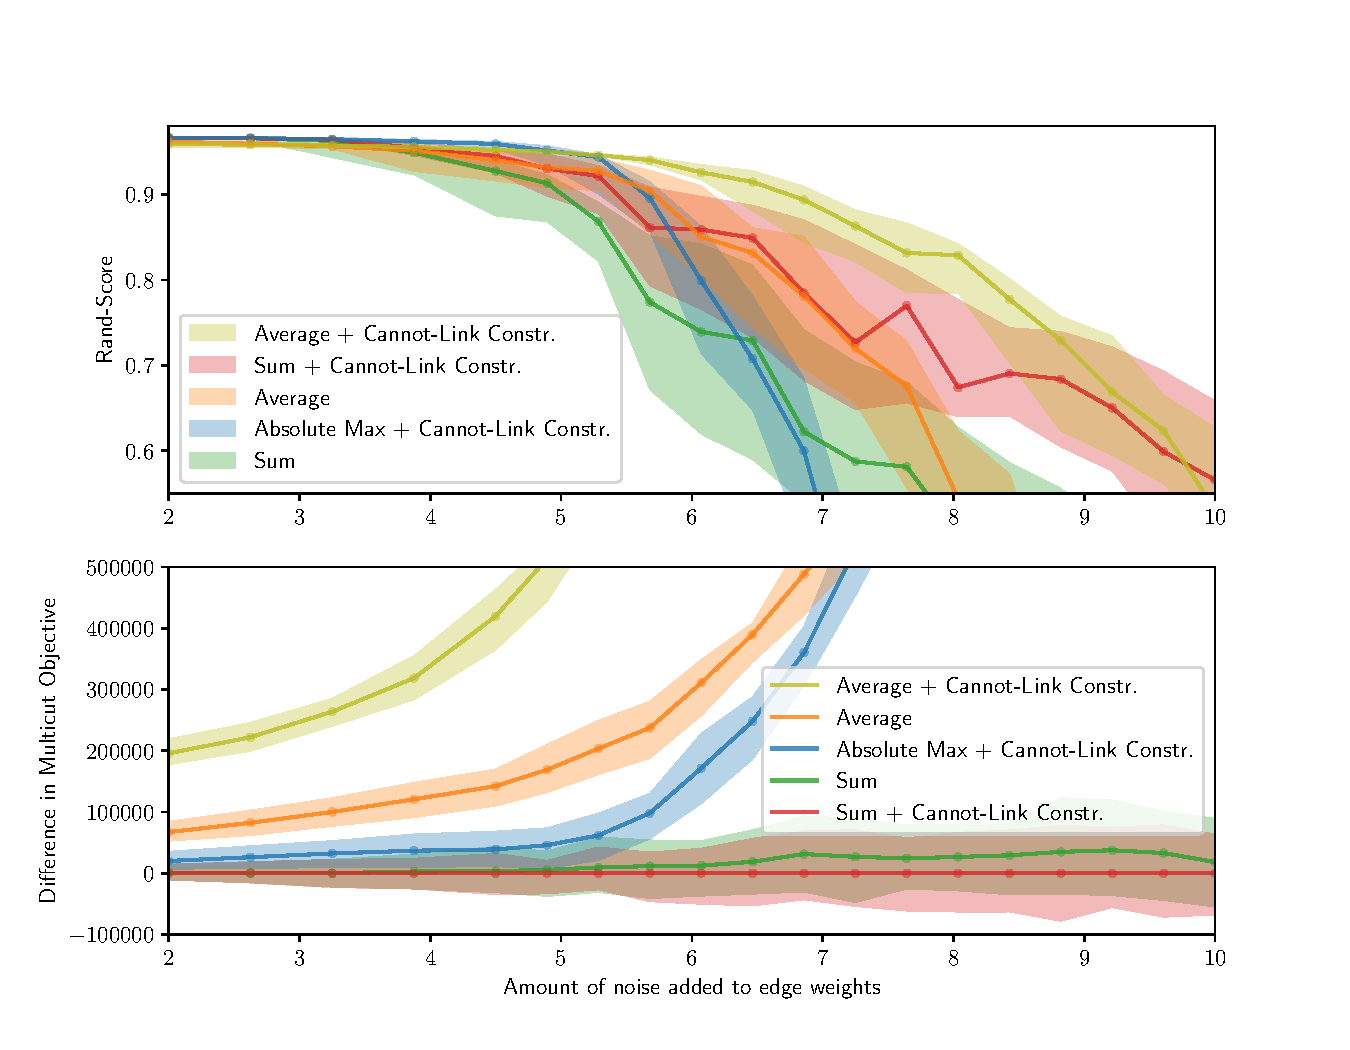
\includegraphics[width=\textwidth,trim=0.55in 0.35in 0.65in 0.80in,clip]{./figs/merge_noise_only_direct.pdf}

    %     \caption{Without long-range edges: $p_{\mathrm{long}}=0$} \label{fig:merge_noise_only_direct}
    % \end{subfigure} \hfill
    % \begin{subfigure}[t]{0.49 \textwidth}
    %     \centering
    %     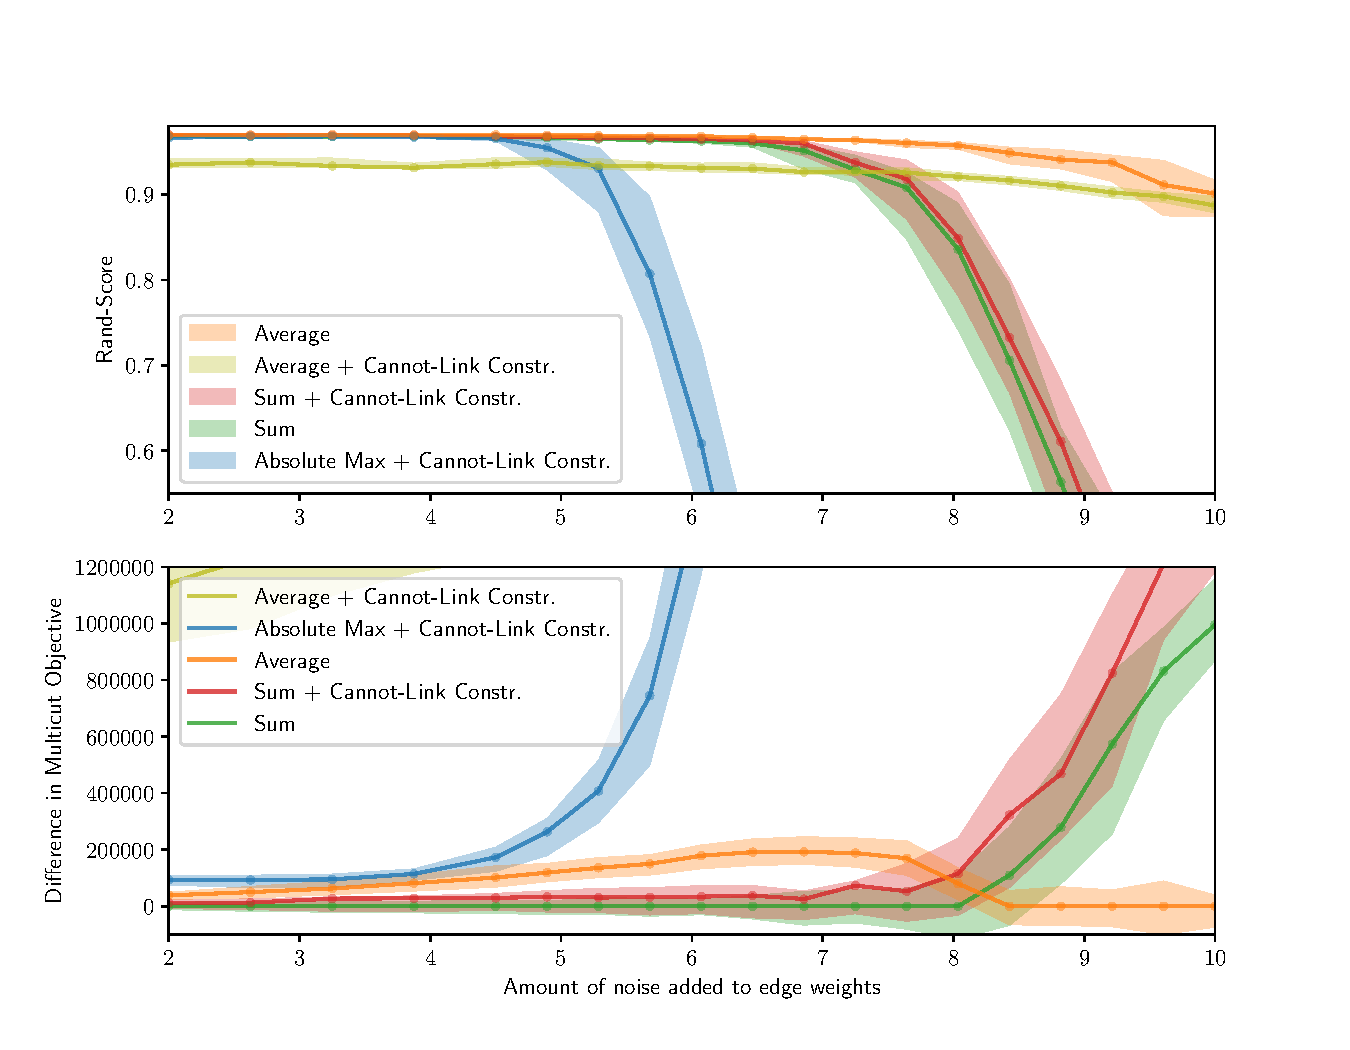
\includegraphics[width=\textwidth,trim=0.53in 0.35in 0.65in 0.80in,clip]{./figs/merge_noise_long_range.pdf}
    %     \caption{With long-range edges: $p_{\mathrm{long}}=0.1$} \label{fig:merge_noise_with_long_range}
    % \end{subfigure}
    \begin{subfigure}[t]{0.49 \textwidth}
        \centering
        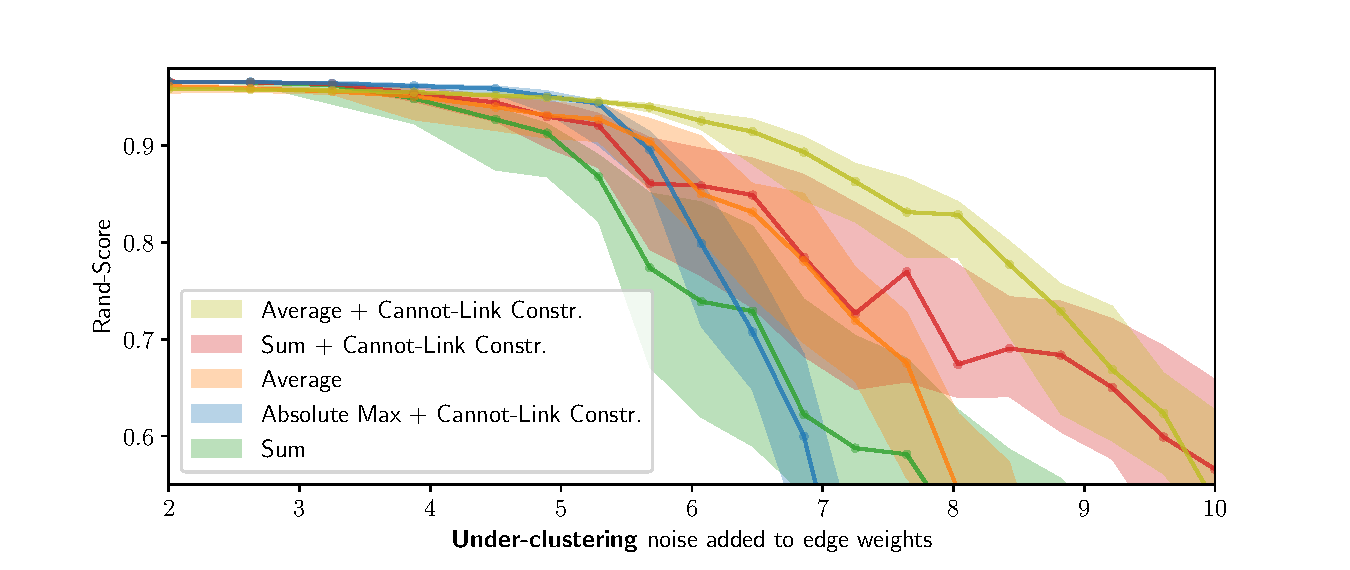
\includegraphics[width=\textwidth,trim=0.55in 0.1in 0.65in 0.45in,clip]{./figs/noise_plots/under_segment_plots_0.pdf}
        % \caption{Without long-range edges: $p_{\mathrm{long}}=0$} \label{fig:merge_noise_only_direct}
    \end{subfigure} \hfill
    \begin{subfigure}[t]{0.49 \textwidth}
        \centering
        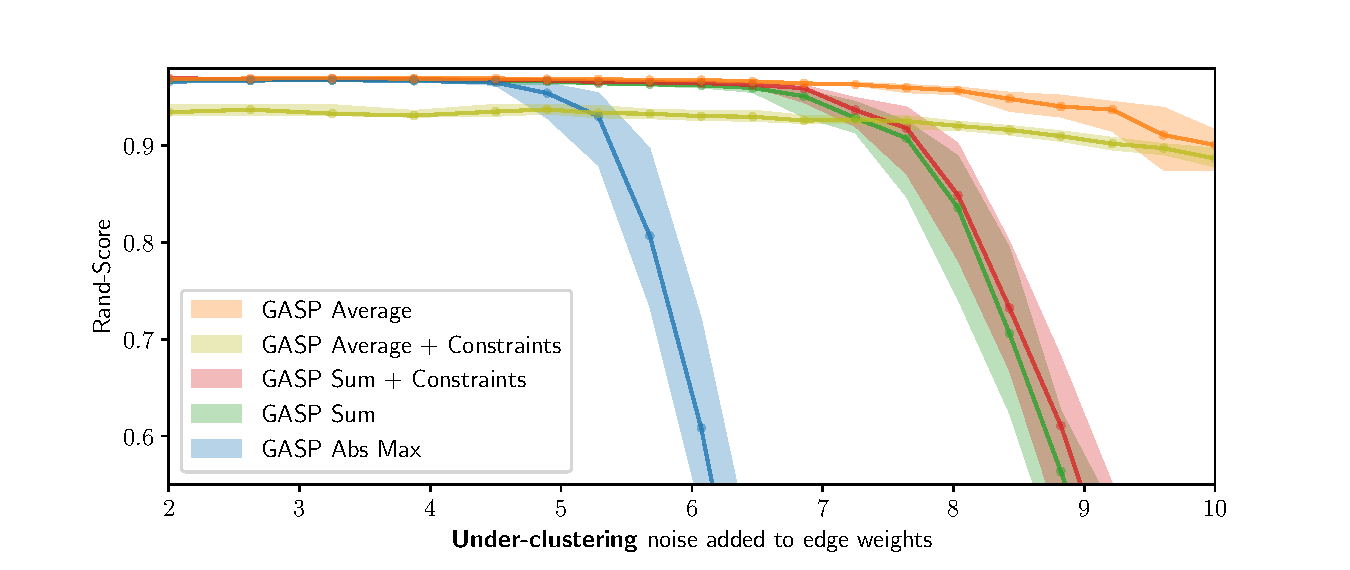
\includegraphics[width=\textwidth,trim=0.53in 0.1in 0.65in 0.45in,clip]{./figs/noise_plots/under_segment_plots_1.pdf}
        % \caption{With long-range edges: $p_{\mathrm{long}}=0.1$} \label{fig:merge_noise_with_long_range}
    \end{subfigure}

        \begin{subfigure}[t]{0.49 \textwidth}
        \centering
        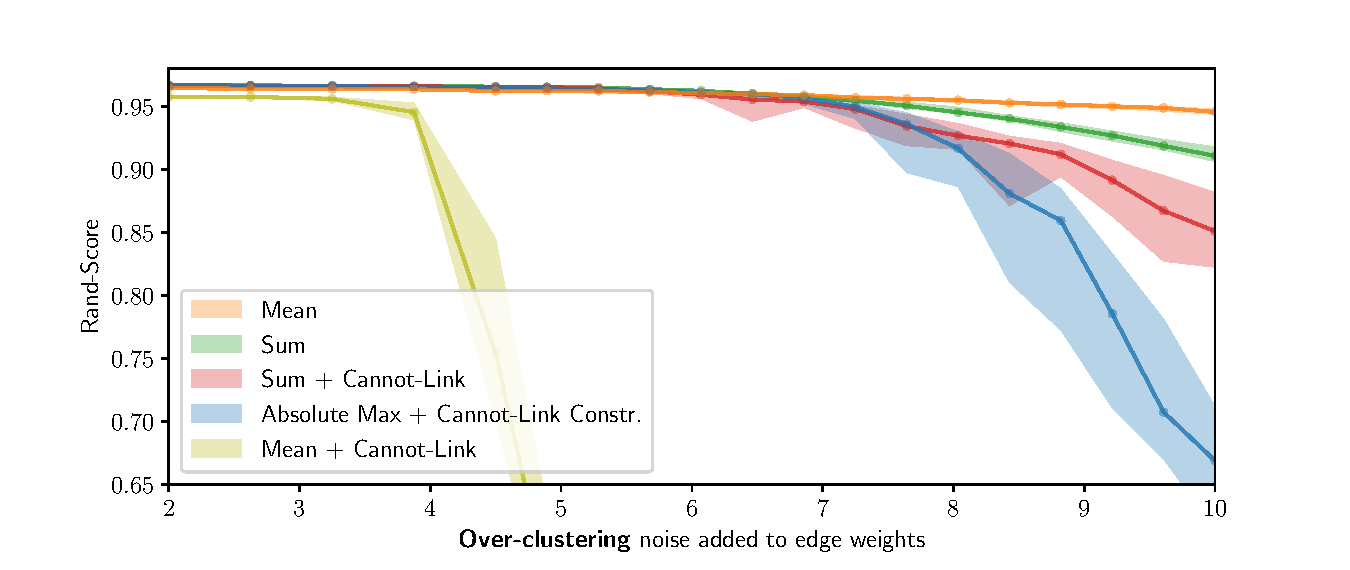
\includegraphics[width=\textwidth,trim=0.55in 0.1in 0.65in 0.2in,clip]{./figs/noise_plots/over_segment_plots_0.pdf}
        \caption{Without long-range edges} \label{fig:merge_noise_only_direct}
    \end{subfigure} \hfill
    \begin{subfigure}[t]{0.49 \textwidth}
        \centering
        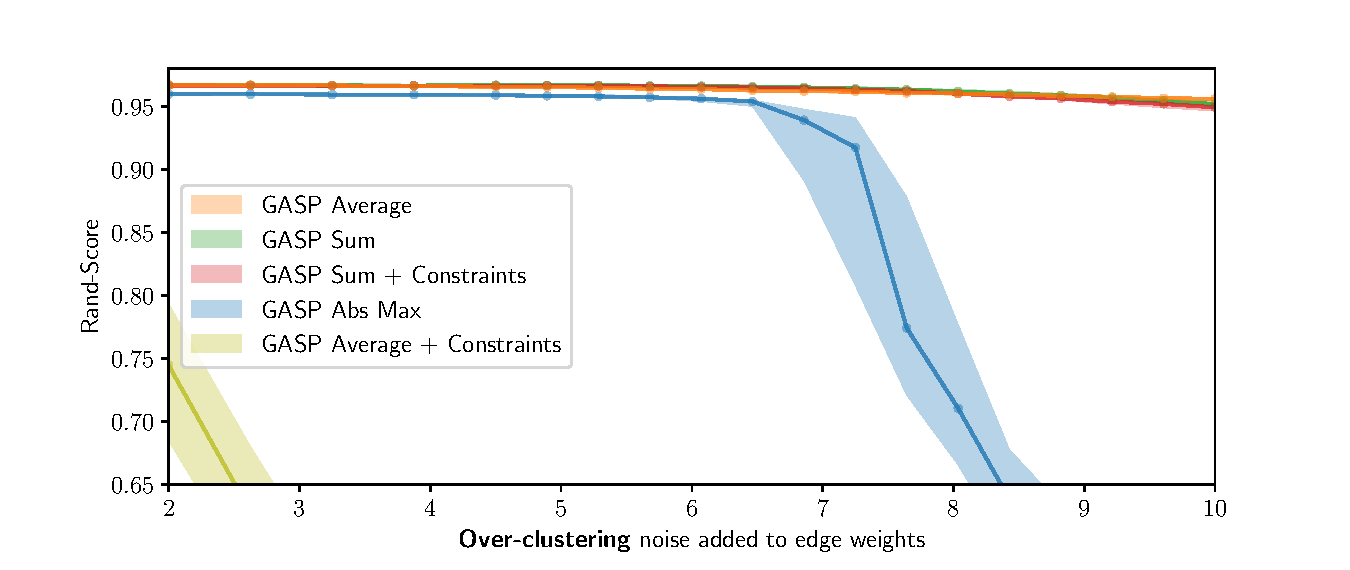
\includegraphics[width=\textwidth,trim=0.53in 0.1in 0.65in 0.20in,clip]{./figs/noise_plots/over_segment_plots_1.pdf}
        \caption{With 10\% long-range edges} \label{fig:merge_noise_with_long_range}
    \end{subfigure}
\caption{\algname{} sensitivity to noise: performances are given by Rand-Score (higher is better) depending on the amount of noise added to the CNN predictions. In all experiments the average linkage proved to be the most robust. Solid lines represent median values over 30 experiments. Values between the 25th and the 75th percentile are shown in shade areas. The two set of experiments using under- and over-clustering noise are summarized in the plots at the top and at the bottom, respectively (see Appendix \ref{sec:appendix_noise_gen} for more details). On the right, 10\% of the long-range CNN predictions were randomly added to the grid-graph. 
%\textbf{Bottom}: Multicut objective (Eq. \ref{eq:multicut_obj}), measuring how balanced the final clusterings are (lower is better); for a clearer comparison, an offset is added to the energy values, so that the method achieving the lowest energy is always assigned to value zero. 
}\label{fig:noise_plots}
\end{figure}
% \begin{minipage}[b]{0.48\textwidth}
% % \begin{figure}
%         % \begin{subfigure}[t]{0.48 \textwidth}
%         \centering
%         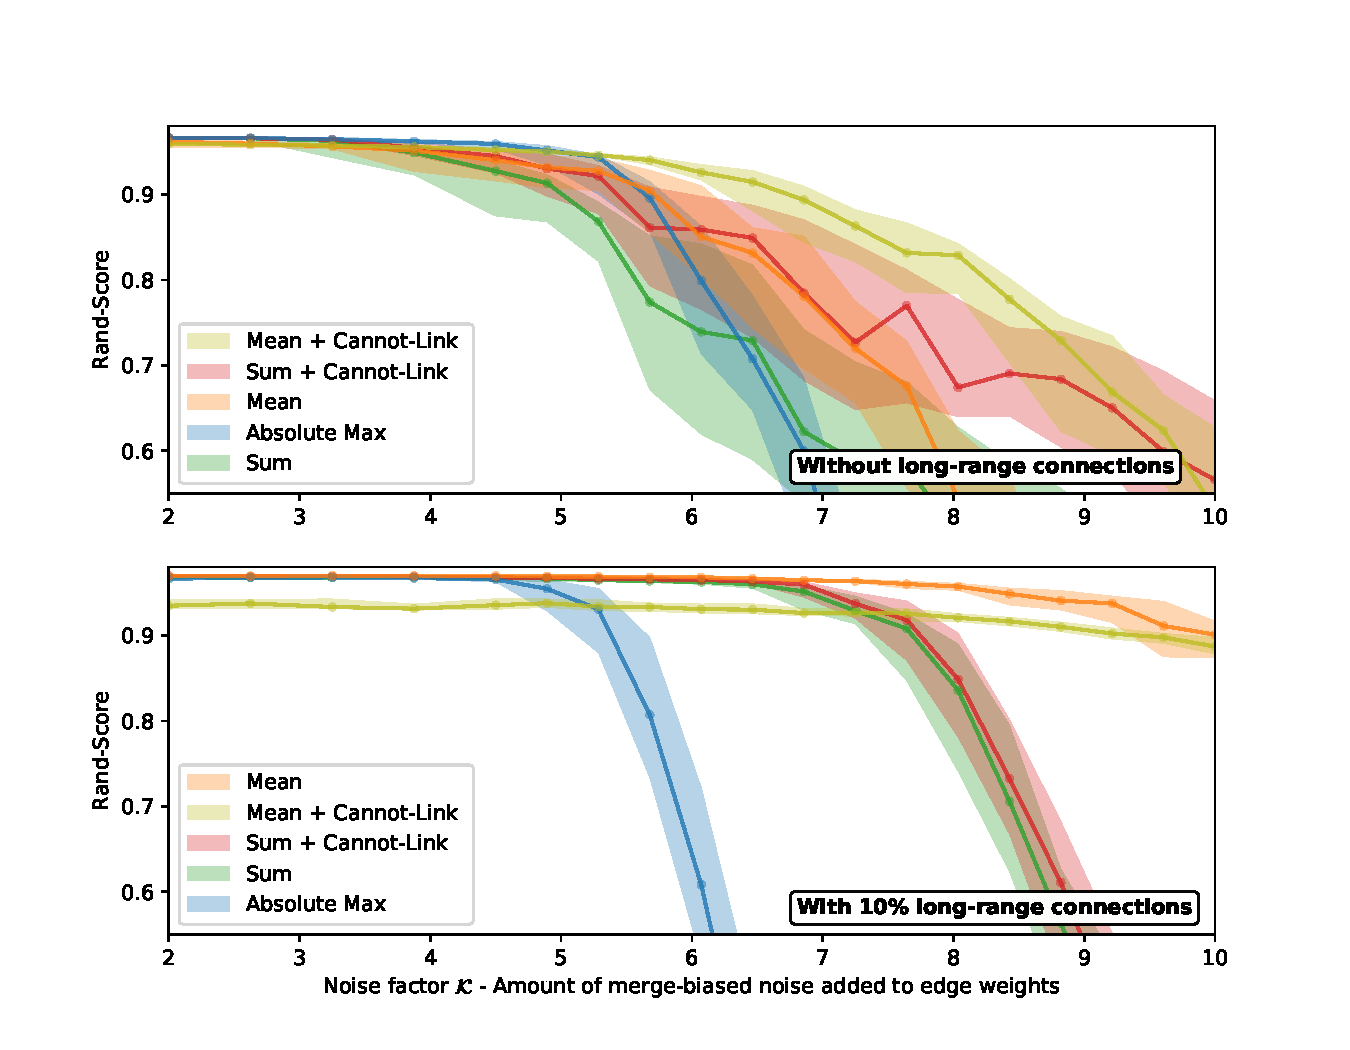
\includegraphics[width=0.98\textwidth,trim=0.35in 0.35in 0.35in 0.35in,clip]{./figs/merge_noise.pdf}
%         \captionof{subfigure}{Merge-biased opensimplex noise} \label{fig:thresh}
%     \end{minipage}\hfil
% \begin{minipage}[b]{0.48\textwidth}
%     % \end{subfigure}%
%     % \begin{subfigure}[t]{0.48 \textwidth}
%         \centering
%         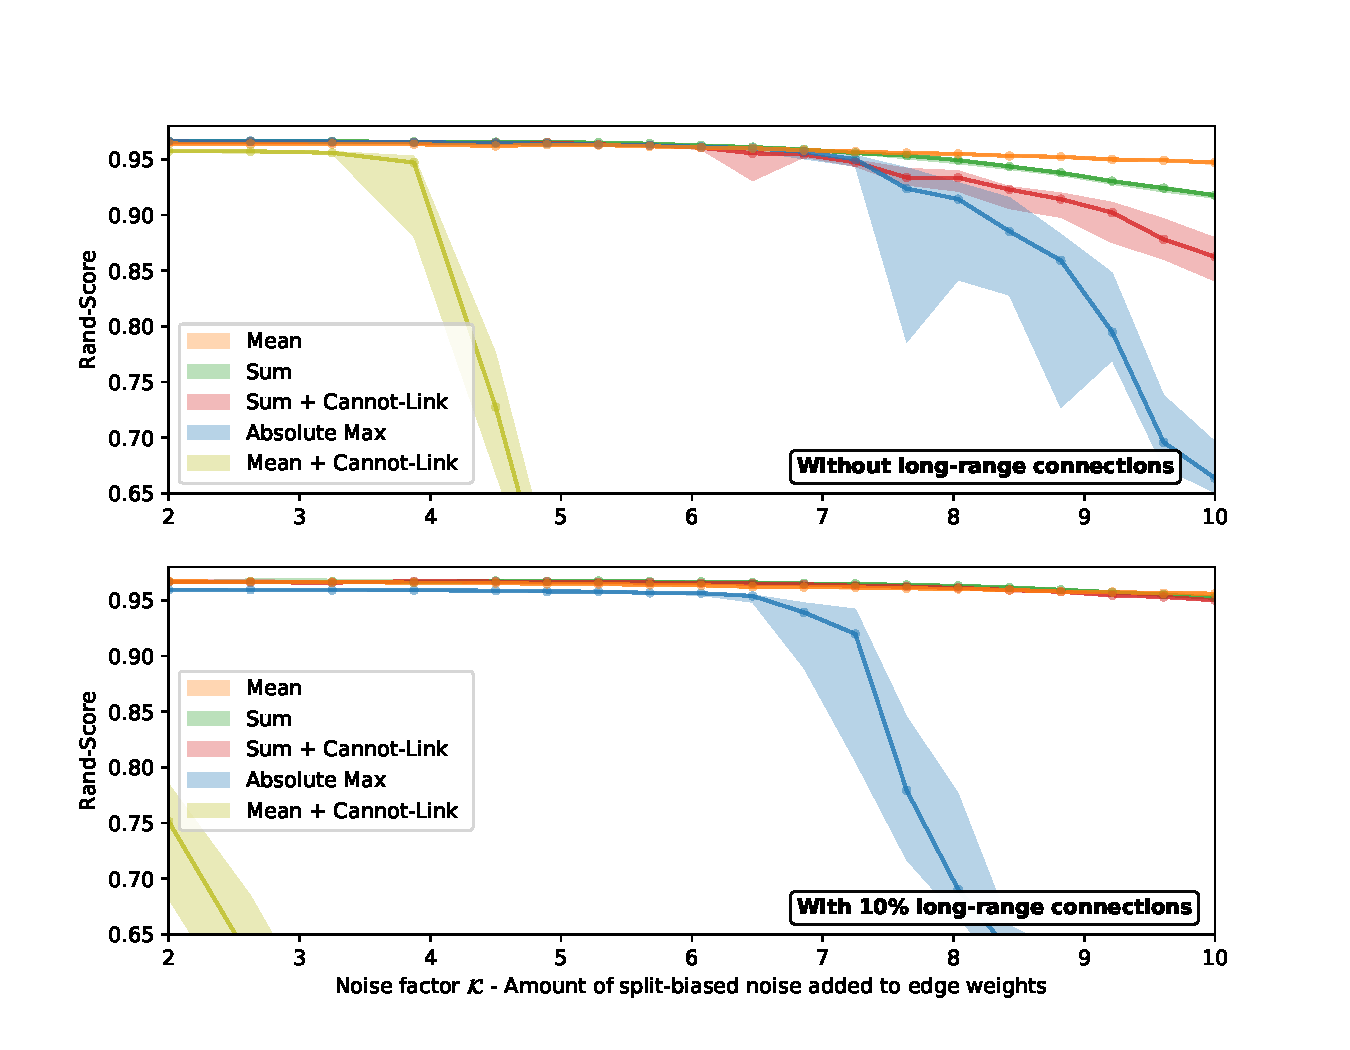
\includegraphics[width=0.98\textwidth,trim=0.29in 0.31in 0.31in 0.31in,clip]{./figs/split_noise.pdf}
%         \captionof{subfigure}{Split-biased opensimplex noise} \label{fig:ws}
%     % \end{subfigure}
% \captionof{figure}{Plot illustrating Adapted RAND scores achieved by UGACA and different update rules when noise is added to the edge weights... Solid lines represent median values, whereas values between the 25th and the 75th percentile are shown in shade areas.    \TODO{Label which uses only local-neighbors and which uses long-range connections}}\label{fig:noise_plots}
% % \end{figure}


\textbf{Noise experiments }  Additionally, we run a set of experiments where the CNN predictions are perturbed by noise, in order to highlight the properties of each \algname{} algorithm and perform an in-depth comparison that is as quantitative as possible. Appendix \ref{sec:appendix_noise_gen} introduces the type of spatially correlated noise that allowed us to perturb the CNN outputs by introducing simulated additional artifacts like missing or false boundary evidences.  
Fig. \ref{fig:noise_plots} summarize our 12000 noise experiments: we focused on the best performing linkage criteria, i.e. \emph{Average}, \emph{Sum} and \emph{Abs Max}, and tested them with different values of noise. %, both with and without use of long-range connections in the grid-graph. % In Fig. \ref{fig:noise_plots}, we used a merge-biased noise decreasing boundary evidence. See Fig. \ref{fig:noise_split} in Appendix for a split-biased version. 

\textbf{Average and Abs Max linkage } Our findings confirm that \algname{} with \emph{Average} linkage criterion represents the most robust algorithm tested and the one that benefits the most from using the long-range CNN predictions. On the other hand, it is not a surprise that the \emph{Abs Max} statistic proposed by \cite{wolf2018mutex} is less robust to noise than the \emph{Average} linkage, but, as we show in the Appendix Table \ref{tab:extended_results_cremi}, \emph{Abs Max} represents a valid and considerably faster option. 
Adding long-range connections to the graph is generally helpful, but when many of them carry repulsive weights, then \algname{} with cannot-link constraints shows a clear tendency to over-cluster.    

\textbf{Sum linkage } 
% The \emph{Sum} linkage generally outputs the most balanced graph partitioning according to the objective defined in Eq. \ref{eq:multicut_obj} and is then confirmed to be a good choice for initializing more complex approximations of the multicut optimization problem like \cite{beier2016efficient}. 
All our experiments show that \algname{} with \emph{Sum} linkage is the algorithm with the highest tendency to under-cluster and incorrectly merge segments (see Fig. \ref{fig:cremi_comparison} for an example). This property is related to the empirical observation that a \emph{Sum} statistic tends to grow clusters one after the other, as shown in Fig. \ref{fig:intro_figure} by the quite unique agglomeration order of the \emph{Sum} statistic. An intuitive explanation of this fact is the following: initially, most of the infra-cluster nodes present similar attractive interactions between each others; when the two nodes sharing the most attractive interaction are merged, there is a high chance that they both share an attractive interaction with a common neighboring node, so the new interaction with this common neighbor will be immediately assigned to a high priority in the agglomeration, given by the sum of two high weights; this usually starts a ``chain reaction'', where only a single cluster is agglomerated at the beginning. On the other hand, as we also see in Fig. \ref{fig:intro_figure}, other linkage criteria like \emph{Average} or \emph{Abs Max} grow clusters of similar sizes in parallel and accumulate in this way much more reliable inter-cluster statistics.





